\documentclass[logo,reportComp]{thesis}
\usepackage[cpp,pseudo]{mypackage}

\title{高级编程技术实验报告}
\subtitle{实验二:Hangman}
\school{数据科学与计算机学院}
\author{陈鸿峥}
\classname{17大数据与人工智能}
\stunum{17341015}
\headercontext{高级编程技术实验报告}
% \authorremark{本实验报告用\LaTeX撰写,创建时间:\builddate\today}

\begin{document}

\maketitle

\section{问题描述及求解思路}
实现一个挂小人(Hangman)的游戏。

\subsection{三个Helper函数}
\begin{itemize}
	\item \verb'is_word_guessed':判断单词是否被猜中\\
	实施方法:采用\verb'for...in...'方法遍历\verb'secret_word'数组,对于每一个字母\verb'c',若\verb'c'不在(用\verb'not...in...'方法)\verb'letters_guessed'中,则说明有字母未被猜中,返回\verb'False';若全部字母都在\verb'letters_guessed'中,则全部字母被猜中,返回\verb'True'
	\item \verb'get_guessed_word':返回带有下划线的猜测单词\\
	实施方法:创建新的空字符串\verb'res',同样遍历\verb'secret_word'的每一个字母\verb'c',若\verb'c'在\verb'letters_guessed'中,则将该字母添加到\verb'res'中;否则用下划线代替
	\item \verb'get_available_letters':返回可用字母\\
	实施方法:对于\verb'letters_guessed'中的每一个字母\verb'c',采用Python内置字符串方法\verb'find'寻找\verb'c'在\verb'ascii_lowercase'字符串中的位置,然后将该位置上的字母剔除,这里采用了\textbf{列表解析}的方法,即
\begin{lstlisting}[language=python]
res = res[:index] + res[index+1:]
\end{lstlisting}
\end{itemize}

\subsection{核心游戏}
游戏规则在problem\_set描述中已经非常详细,这里不再赘述。

实施方法如下:
\begin{itemize}
	\item 初始化计数器\verb'cnt'用来记录用户剩余的``生命'',初始值为6
	\item 如果\verb'cnt'的值大于0,则进入\verb'while'循环
	\item 输出用户提示信息
	\item 根据用户输入的字母进行条件判断:若输入非字母,而是其他字符,则对用户进行提醒(warning),若提醒次数使用完则声明减1
	\item 将字母转换为小写
	\item 判断该字母是否已经猜过,提醒警告规则与4相同,但提示信息不同
	\item 将该字母添加入\verb'guessed'中
	\item 判断是否猜中单词中的字母,若猜中则再判断是否猜完单词,若猜完则游戏结束,输出分数;否则猜元音生命减2,猜辅音生命减1
\end{itemize}

\subsection{带提示的游戏}
两个辅助函数
\begin{itemize}
	\item \verb'match_with_gaps':判断是否匹配带下划线的单词,其中下划线为通配符(widecard)\\
	实施方法:用\verb'strip'函数预处理,去除\verb'my_word'首尾多余空格,先判断字符串长度是否相等,不相等肯定不匹配;然后遍历每一个字符,如果对于每一个字符\verb'my_word'和\verb'other_word'对应位置都相同,或\verb'my_word'采用了通配符,则匹配成功,否则匹配失败
	\item \verb'show_possible_matches':将所有可能的匹配输出\\
	实施方法:用\verb'for...in...'方法遍历\verb'wordlist'中每一个单词\verb'word',调用\verb'match_with_gaps'函数判断\verb'my_word'和\verb'word'是否匹配,如果匹配则输出
\end{itemize}

完整游戏实施只需在上一题的基础上,在输入字符后判断是否为\verb'*',如果是则调用\verb'show_possible_matches'函数,将所有可能匹配输出,作为提示。

\section{代码}
代码实施及注释请见附件\verb'hangman.py'。

\section{运行截图}
实验运行结果如下面几幅图片所示,注意图中\textbf{将游戏规则中的各种情况都进行了测试,也包括自定义的极端样例},且结果正确。
\begin{figure}[H]
\centering
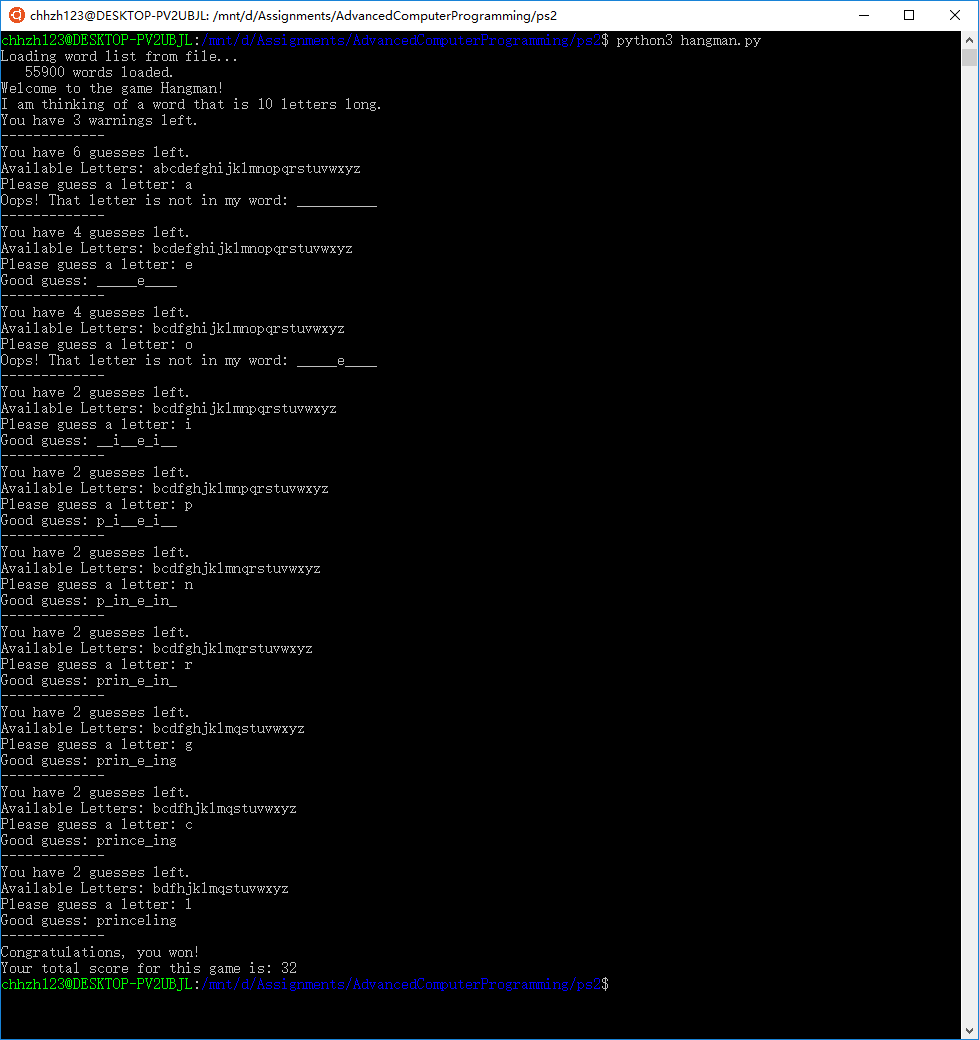
\includegraphics[width=\linewidth]{fig/win_no_hint.PNG}
\caption{无提示,游戏胜利}
\end{figure}
\begin{figure}[H]
\centering
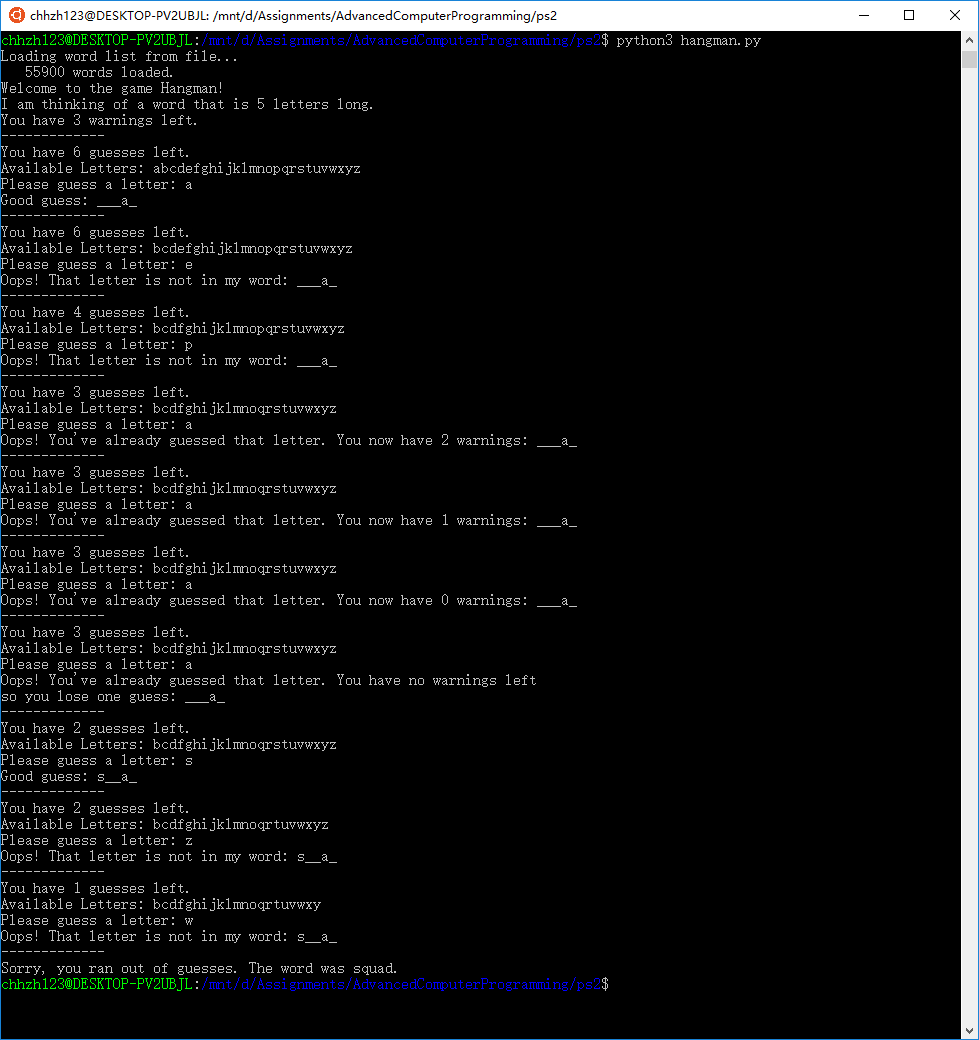
\includegraphics[width=\linewidth]{fig/lose_no_hint.PNG}
\caption{无提示,游戏失败}
\end{figure}
\begin{figure}[H]
\centering
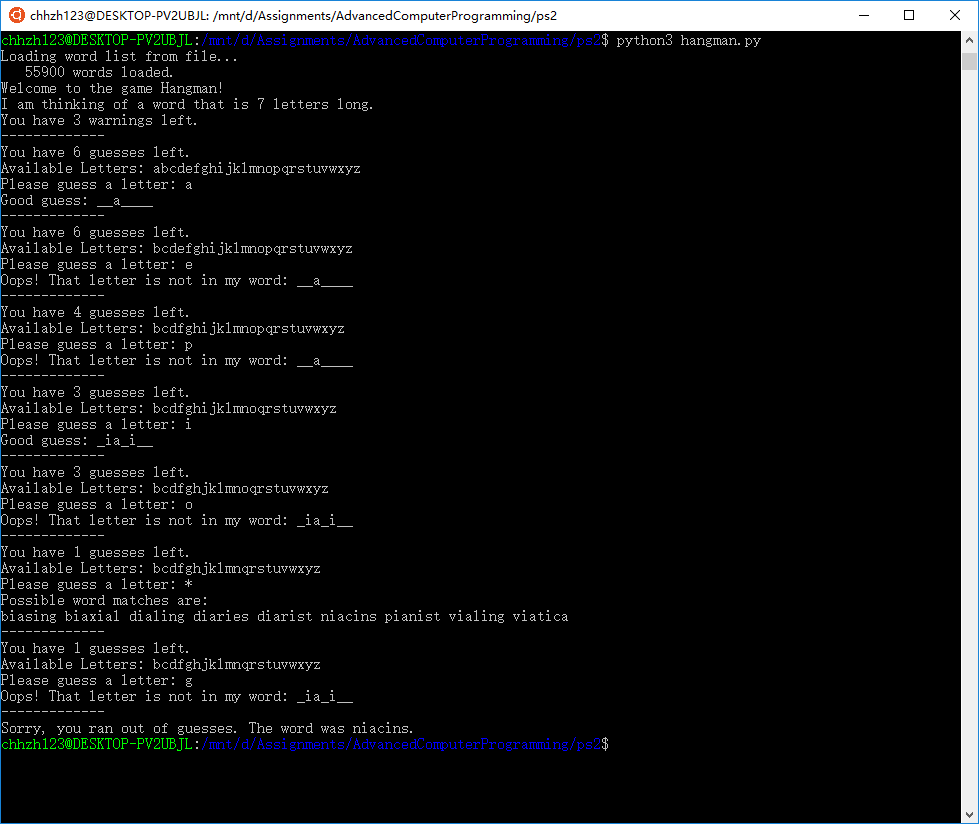
\includegraphics[width=\linewidth]{fig/hint.PNG}
\caption{带提示的游戏}
\end{figure}

\end{document}

% 实验提交内容
% 邮件主题,作业文件命名规范(学号、姓名)
% 文档pdf格式(问题、求解思路、代码、注释、运行截图)
% 考虑健壮性、可读性
% 极端样例